\documentclass[11pt,a4paper]{article}

\usepackage[utf8]{inputenc}
\usepackage[margin=1in]{geometry}
\usepackage{amsmath,amssymb}
\usepackage{graphicx}
\usepackage{booktabs}
\usepackage{tabularx}
\usepackage{hyperref}
\usepackage{caption}
\usepackage{subcaption}
\usepackage{float}
\usepackage{microtype}
\usepackage{enumitem}
\usepackage{xcolor}
\usepackage{listings}

\hypersetup{
    colorlinks=true,
    linkcolor=blue!70!black,
    citecolor=blue!70!black,
    urlcolor=blue!70!black
}

\lstset{
    basicstyle=\ttfamily\footnotesize,
    breaklines=true,
    frame=single,
    backgroundcolor=\color{gray!10},
    keywordstyle=\color{blue}\bfseries,
    commentstyle=\color{green!50!black}\itshape,
    stringstyle=\color{red!60!black}
}

\title{\textbf{\Large Changing Patterns of Occupation, Ecological Niches, and Socio-Economic Interdependence in Chamba District (1881--1961)}\\[0.3em]
}

\author{
    \textbf{Bala Subramanian} \and 
    \textbf{Vagdevi Reddy} \and 
    \textbf{Phanindra} \\[0.5em]
}
\begin{document}
\date{} % Removes the date

\maketitle

\begin{abstract}
This report presents the computational methodology, source harmonization, and empirical findings for our historical investigation into Chamba District, Himachal Pradesh. Investigating how changing patterns of occupation shaped caste and religious relations from the late nineteenth century to 1961 across Brahmaur, Chitrari, and Maingal. Rather than treating colonial censuses and village monographs as passive repositories, we apply Optical Character Recognition (OCR), ink-density connected-blob image detection, Devanagari oral poetry mining, Keyword-in-Context (KWIC) concordance extraction, and relative word frequency normalization (mentions per 1,000 words). We reconstruct two source-linked datasets (Dataset A: 25 quantitative records; Dataset B: 20 verbatim qualitative passages) and a 12-relationship bipartite exchange matrix. Our computational and archival analysis demonstrates that: (1) environmental altitude imposed strict physiological ceilings on pastoral production, barring water buffaloes from alpine Brahmaur due to severe cold-induced lactation collapse (dropping from 9 to 4 seers/day) and restricting them to sub-Himalayan Maingal; (2) village-level caste divisions of labour were tightly specialized rather than generic, with Sipis holding a tripartite monopoly in Brahmaur as wage shepherds (\textit{pohals}), tweed weavers, and \textit{Nawala} ritual drummers, while attached Halis mobilized as \textit{Aryas--Halis} in Chitrari, and Lohar blacksmiths received non-monetary \textit{khalian} threshing-floor grain shares in Maingal; and (3) inter-religious co-existence between Muslim Gujjars and Hindu Brahmins was anchored in non-competing ecological niches (forest buffalo dairying versus terraced arable cultivation).
\end{abstract}

\vspace{0.5em}
\noindent\textbf{Keywords:} Himalayan Pastoralism, Transhumance, Gaddis, Gujjars, Ecological Ceiling, Jajmani Barter, Computational History, OCR, Text Mining, Chamba State.

\newpage
\tableofcontents
\newpage

\section{Introduction and Historiographical Problem}

\subsection{The Research Problem}
Mountain societies in the Western Himalayas have frequently been depicted in colonial gazetteers and popular memory as static, timeless isolates governed by rigid caste hierarchies. This project investigates the historical transition of the upper Ravi River basin of Chamba District, Himachal Pradesh, from the late nineteenth century to 1961. Our central research question asks:
\begin{quote}
\textit{How did changing patterns of occupation and economic interdependence shape caste and religious relations in Brahmaur, Chitrari, and Maingal from the late nineteenth century to 1961?}
\end{quote}

We examine this transition across three distinct micro-ecological and social settings:
\begin{enumerate}[leftmargin=*]
    \item \textbf{Brahmaur (Brahmaur Sub-Tehsil / Gaderan, $\sim$7,000 ft):} An alpine valley characterized by Gaddi sheep and goat pastoralism, trans-Himalayan seasonal migration across the Dhaula Dhar and Pir Panjal ranges, the sacred Chaurasi temple complex, and institutionalized service relations between upper-caste Gaddi flock owners (Rajputs/Brahmins) and lower-caste artisans (Sipis, Reharas).
    \item \textbf{Chitrari (Chamba Tehsil, $\sim$5,800 ft):} An intermediate terraced river basin dominated by landed Brahmin hegemony (77\% of the population) tied to the historic Shakti Devi temple endowment, intensive plough agriculture, attached ploughmen labour (\textit{Halis}, later mobilizing as \textit{Aryas}), and seasonal milk trade with transhumant pastoralists.
    \item \textbf{Maingal (Chamba Tehsil, $\sim$4,000 ft):} A sub-Himalayan forested slope presenting a multi-religious frontier where settled Muslim Gujjar buffalo pastoralists living in dispersed forest \textit{kothas} co-existed and exchanged goods and services with sedentary Hindu Brahmins, Rajputs, and blacksmith artisans (\textit{Lohars}).
\end{enumerate}

\subsection{Theoretical Framework: Marxist and the Annales Methods}
Our historical inquiry synthesizes two complementary paradigms:
\begin{itemize}[leftmargin=*]
    \item \textbf{Historical Materialism:} We trace how the material conditions of production-pasture permits, terraced landholdings, livestock herds, and iron agricultural implements-structured the social division of labour. We examine how non-monetary customary barters (\textit{khalian} grain sheaves, sacrificial meat shares) persisted alongside expanding market commodities (commercial ghee marketing, contractual shepherd wages).
    \item \textbf{The Annales School (\textit{Longue Durée} and Ecological History):} We treat geographical relief, altitudinal zonation, winter snowlines, and animal biology as active structures that established physiological ceilings on pastoral strategies and dictated the rhythms of seasonal transhumance.
    \item \textbf{Critical Deconstruction of the Colonial Archive:} We treat British imperial censuses (Ibbetson 1881; Middleton 1931) and ethnographic glossaries (Rose 1911--1919) not as neutral compendia of facts, but as colonial classification projects that essentialized mobile hill communities into fixed racial and occupational categories.
\end{itemize}

---

\section{Source Corpus and Administrative Hierarchy}

To analyze social relations rigorously, primary historical evidence must be interpreted at its proper administrative and geographic scale. Historical documentation in the Western Himalayas operates across a four-tiered hierarchy:

\[
\begin{aligned}
&\text{British Punjab Province}
\longrightarrow \text{Chamba Princely State (Macro)}\\
&\longrightarrow \text{Tehsils / Wazarats}
\longrightarrow \text{Villages / Hamlets (Micro)}
\end{aligned}
\]


Our corpus integrates macro-colonial demographic returns with post-independence micro-household monographs (Table~\ref{tab:sources}).

\begin{table}[H]
\centering
\small
\caption{Primary Archival Source Inventory and Geographic Resolution}
\label{tab:sources}
\begin{tabularx}{\textwidth}{llcp{3.2cm}X}
\toprule
\textbf{Source Tag} & \textbf{Historical Period} & \textbf{Year} & \textbf{Administrative Level} & \textbf{Analytical Focus and Character} \\
\midrule
Census 1881 & Late 19th Century & 1881 & Punjab Province / Chamba State & Denzil Ibbetson's census; ethnographic paternalism; bi-regional landholding across Dhaula Dhar. \\
Rose 1919 & Early 20th Century & 1911--19 & Punjab Province \& NWFP & H. A. Rose's Glossary; fourfold Gaddi caste taxonomy; pejorative pastoral stereotypes. \\
Census 1931 & Interwar Depression & 1931 & Punjab States / Chamba State & Vol. XVII Pt. 1; tripartite economic shift (Earners, Working Dependents); rural household density. \\
Brahmaur 1961 & Post-Independence & 1961 & Village Monograph No. 5 & Micro-census of 136 households (721 pop); 4,484 sheep/goats; Sipi artisanal monopoly; \textit{Nawala} ritual. \\
Chitrari 1961 & Post-Independence & 1961 & Village Monograph No. 10 & Micro-census of 80 households (404 pop); 77\% Brahmin; attached Halis (\textit{Aryas}); temple economy. \\
Maingal 1961 & Post-Independence & 1961 & Village Monograph No. 27 & Micro-census of 41 households (249 pop across 13 hamlets); 217 buffaloes; Muslim Gujjar dairy economy. \\
\bottomrule
\end{tabularx}
\end{table}



\section{Computational Methodology and Pipeline Architecture}

To extract, normalize, and analyze the bilingual English-Devanagari corpus, we developed an end-to-end computational pipeline.

\begin{figure}[H]
\centering
\fbox{
\begin{minipage}{0.92\textwidth}
\small
\textbf{Computational Pipeline Workflow:}
\begin{enumerate}[leftmargin=*]
    \item \textbf{Decryption and Sanitization:} PDF repair and decryption using \texttt{qpdf}; standardized indexing of archival volumes across collections.
    \item \textbf{Multi-Lingual OCR Layer:} Tesseract OCR multi-threaded engine configured with bilingual language models (\texttt{-l eng+hin} and \texttt{-l eng+urd+hin}) generating searchable text while preserving character coordinates.
    \item \textbf{Connected-Blob Image Extraction:} Rendering scanned pages at 50 DPI grayscale, masking text bounding boxes, and executing connected-component ink-density analysis to extract 140 technical line drawings, maps, and photographs.
    \item \textbf{Devanagari Oral History Mining:} Filtering scanner smudges using Unicode Devanagari character-ratio thresholds to isolate 366 lines of vernacular Pahari folk ballads.
    \item \textbf{Timeline-Specific Computational Modules:}
    \begin{itemize}
        \item \textbf{1881 Imperial Census Analysis:} Concordance extraction for Gaddi and Gujjar transhumance and dual-tenure landholding across the Dhaula Dhar.
        \item \textbf{1911--1919 Ethnographic Glossary Analysis:} Extraction of caste taxonomies and automated auditing of colonial bias vocabulary.
        \item \textbf{1931 Interwar Census Analysis:} Extraction of Chamba State demographic aggregates and economic dependency ratios.
        \item \textbf{1961 Village Surveys Micro-Analysis:} Lexical normalization per 1,000 words and Keyword-in-Context (KWIC) interaction extraction.
    \end{itemize}
    \item \textbf{Visualization Rendering:} Algorithmic rendering of publication-grade figures at 300 DPI.
\end{enumerate}
\end{minipage}
}
\caption{System Architecture of the Computational Pipeline}
\label{fig:pipeline}
\end{figure}

---

\section{Timeline-Specific Computational Analysis}

\subsection{1881 Punjab Census Analysis}
Our computational analysis processes 6 volumes (over 696,000 searchable words) of Denzil Ibbetson's 1881 Census. Using targeted regular expression patterns, we extract 718 concordance records demonstrating the paternal-ethnographic framework of early colonial rule:
\begin{itemize}[leftmargin=*]
    \item \textbf{Bi-Regional Land Tenure:} Paragraph 498 reveals that Gaddis held land simultaneously in Kangra (British territory) for winter wheat cropping and in Brahmaur (Chamba Princely State) for summer grazing, paying grazing dues to both authorities.
    \item \textbf{Generic Classification:} Ibbetson recorded that while \textit{Gaddi} was applied generically by plains observers, impure service castes (Sipis, Halis, Badis) were excluded from the inner core of the Gaddi designation.
\end{itemize}

\subsection{1911--1919 H. A. Rose Glossary Analysis}
Our text mining pipeline parses Rose's multi-volume compendium (over 789,000 words), generating 387 ethnographic concordance records and systematically auditing colonial bias:
\begin{itemize}[leftmargin=*]
    \item \textbf{Racial Stratification:} Rose codified a fourfold hierarchical taxonomy of Gaddis, asserting that upper Gaddis were immigrant Khatris fleeing Mughal persecution, while lower service groups were menials.
    \item \textbf{Criminalization of Pastoralists:} Computational analysis identifies pejorative proverbs recorded by colonial administrators, which characterized Gujjars as ``lazy cultivators and habitual cattle thieves.''
\end{itemize}

\subsection{1931 Punjab Census Analysis}
Computational parsing of Vol. XVII and Part I of the 1931 Census (338,000 words) extracts 560 concordances and 28 Chamba State demographic baseline records:
\begin{itemize}[leftmargin=*]
    \item \textbf{Shift to Economic Dependency:} Under the impact of the Great Depression, the census abandoned hereditary caste ascriptions to record \textit{Principal Earners}, \textit{Working Dependents}, and \textit{Non-Working Dependents}.
    \item \textbf{Chamba State Macro-Baseline:} In Chamba State, 30,665 occupied houses were returned across a rural population of 146,870 (average household density of 4.79 persons per house).
\end{itemize}

\subsection{1961 Village Surveys Micro-Analysis}
Rather than aggregating the 1961 surveys as an undifferentiated regional whole, our computational analysis processes each village monograph individually, extracting local demographic tables, livestock enumerations, and qualitative excerpts before performing comparative normalization.

\subsubsection{Brahmaur Alpine Micro-Historical Analysis}
Processing Monograph No.~5 (65,302 words) yields 12 quantitative records and 5 verbatim passages:
\begin{itemize}[leftmargin=*]
    \item \textbf{Demographic Structure:} 55 Rajput households (293 persons; 40.6\%) and 48 Brahmin households (251 persons; 34.8\%) form the landed and priestly core; 15 Sipi households (119 persons; 16.5\%) represent the artisan base (Village Census, 1961).
    \item \textbf{Livestock Censuses:} 4,484 sheep and goats owned across 48 households; 0 water buffaloes due to cold-induced lactation drop from 9 to 4 seers (Brahmaur Survey, p.~43).
    \item \textbf{Labour Stratification:} Differentiates owner-shepherds (\textit{malundi}) from contractual wage-shepherds (\textit{pohal}) receiving food, clothing, wool, a 2--4\% sheep dividend, and Rs.~2/month cash (Brahmaur Survey, pp.~38,~44).
\end{itemize}

\subsubsection{Chitrari Basin Micro-Historical Analysis}
Processing Monograph No.~10 (41,363 words) yields 7 quantitative records and 4 verbatim passages:
\begin{itemize}[leftmargin=*]
    \item \textbf{Temple Hegemony:} Landed Brahmins comprise 77\% of the sample (311 persons across 60 households), their dominance originating from historic royal land endowments by Raja Meru-Varman (Chitrari Survey, p.~7).
    \item \textbf{Agrarian Tenancy and Social Mobility:} 2 households of attached Halis (6 persons) cultivate Brahmin land under customary plough service, while actively mobilizing under the Arya Samaj as \textit{Aryas--Halis} (Chitrari Survey, pp.~11--12).
    \item \textbf{Sedentary Cattle Focus:} 155 oxen for terraced ploughing; only 123 sheep and 36 goats, contrasting with Brahmaur's transhumance (Chitrari Survey, p.~42).
\end{itemize}

\subsubsection{Maingal Slopes Micro-Historical Analysis}
Processing Monograph No.~27 (70,551 words) yields 4 quantitative records and 4 verbatim passages:
\begin{itemize}[leftmargin=*]
    \item \textbf{Muslim Gujjar Predominance:} 203 Muslim Gujjars (25 households; 81.5\% of the surveyed population) live in 13 dispersed forest hamlets in flat-roofed \textit{kothas} (Maingal Survey, p.~12).
    \item \textbf{Commercial Dairy Herd:} 217 water buffaloes producing clarified butter (\textit{ghee}) marketed in Chamba town bazaar (Maingal Survey, pp.~14,~33).
    \item \textbf{Jajmani Blacksmith Barter:} 2 Lohar households (8 persons) repair iron ploughshares in exchange for non-monetary \textit{khalian} unhusked grain sheaves delivered directly from harvest threshing floors (Maingal Survey, pp.~12,~33).
\end{itemize}

\subsection{Cross-Scale Harmonization and Comparative Integration}
Following localized extraction across individual historical sources and village monographs, our comparative framework harmonizes the disparate data layers:
\begin{enumerate}[leftmargin=*]
    \item \textbf{Unified Multi-Scale Datasets:} Synthesizes quantitative demographic returns (25 verified records) and verbatim qualitative evidence (20 contextual excerpts) into structured relational schemas across all three administrative levels.
    \item \textbf{Cross-Period Comparability Crosswalk:} Systematically maps categorical drift across eras---tracing the transition from 1881 paternal caste classifications, through 1931 depression dependency categories, to 1961 village-level occupational returns.
    \item \textbf{Cross-Village Word Frequency Normalization:} Computes normalized relative frequencies (mentions per 1,000 words):
    \[
    \text{Normalized Frequency} = \left( \frac{\text{Absolute Keyword Hits}}{\text{Total Searchable Words}} \right) \times 1,000
    \]
    enabling direct mathematical comparison across different monograph lengths (Table~\ref{tab:frequencies}).
\end{enumerate}

---

\section{Empirical Findings: Comparative Analysis Across Villages and Historical Periods}

\begin{enumerate}[leftmargin=*]
    \item \textbf{Cross-Village Spatial \& Ecological Comparison (1961):} Comparing Brahmaur ($\sim$7,000 ft), Chitrari ($\sim$5,800 ft), and Maingal ($\sim$4,000 ft) across ecological altitudinal ceilings, livestock endowments, artisan service divisions, and inter-religious co-existence.
    \item \textbf{Longitudinal Cross-Period Historical Comparison (1881--1961):} Tracing the shift from early colonial paternal-caste taxonomies (Ibbetson 1881), through pejorative ethnographic stereotypes (Rose 1911--1919) and depression-era dependency models (1931), to post-independence village-level socio-economic realities (1961).
\end{enumerate}

Each comparative finding follows our required analytical progression:
\[
\begin{aligned}
\text{Observation} &\longrightarrow \text{Source Verification} \longrightarrow \text{Comparison} \\
&\longrightarrow \text{Interpretation} \longrightarrow \text{Alternative Explanation} \longrightarrow \text{Limitation}
\end{aligned}
\]

\begin{table}[H]
\centering
\small
\caption{Normalized Relative Word Frequencies Across 1961 Village Monographs (Mentions per 1,000 Words)}
\label{tab:frequencies}
\begin{tabularx}{\textwidth}{lcrrrX}
\toprule
\textbf{Category} & \textbf{Lemma} & \textbf{Brahmaur} & \textbf{Chitrari} & \textbf{Maingal} & \textbf{Primary Census Grounding} \\
\midrule
\textbf{Sheep} & \texttt{sheep} & \textbf{1.240} & 0.919 & 0.312 & 4,484 sheep in Brahmaur vs 123 in Chitrari \\
\textbf{Gaddi} & \texttt{gaddi} & \textbf{2.067} & 1.402 & 0.780 & Gaddis dominate Brahmaur population \\
\textbf{Gujjar} & \texttt{gujjar} & 0.000 & 0.048 & \textbf{2.750} & 203 Muslim Gujjars (81.5\%) in Maingal \\
\textbf{Buffalo} & \texttt{buffalo} & 0.138 & 0.073 & \textbf{0.354} & 0 kept in Brahmaur vs 217 in Maingal \\
\textbf{Temple} & \texttt{temple} & \textbf{2.358} & 1.596 & 0.142 & Chaurasi (Brahmaur) \& Shakti Devi (Chitrari) \\
\textbf{Muslim} & \texttt{muslim} & 0.123 & 0.000 & \textbf{0.595} & 1 hh in Brahmaur vs 25 hh in Maingal \\
\textbf{Nawala / Shiva} & \texttt{shiva/nawala} & \textbf{0.995} & 1.015 & 0.014 & Sacrificial Shaivite feasts in Brahmaur \& Chitrari \\
\textbf{Brahmin} & \texttt{brahmin} & 0.276 & 0.725 & \textbf{1.219} & 77\% in Chitrari; ethnographer comparison in Maingal \\
\textbf{Rajput} & \texttt{rajput} & \textbf{0.582} & 0.363 & 0.312 & 293 pop (40.6\%) in Brahmaur \\
\textbf{Sipi} & \texttt{sipi} & \textbf{0.720} & 0.024 & 0.000 & 119 pop in Brahmaur; specialized artisans \\
\textbf{Hali} & \texttt{hali} & 0.031 & \textbf{0.193} & 0.000 & Attached ploughmen in Chitrari \\
\textbf{Lohar} & \texttt{lohar} & 0.015 & 0.097 & \textbf{0.312} & Blacksmith \textit{khalian} barter in Maingal \\
\textbf{Land} & \texttt{land} & \textbf{1.608} & 1.233 & 0.737 & Universal arable baseline \\
\textbf{Maize} & \texttt{maize} & \textbf{0.704} & 0.798 & 0.581 & Universal dietary staple across middle Ravi valley \\
\bottomrule
\end{tabularx}
\end{table}

\begin{figure}[H]
\centering
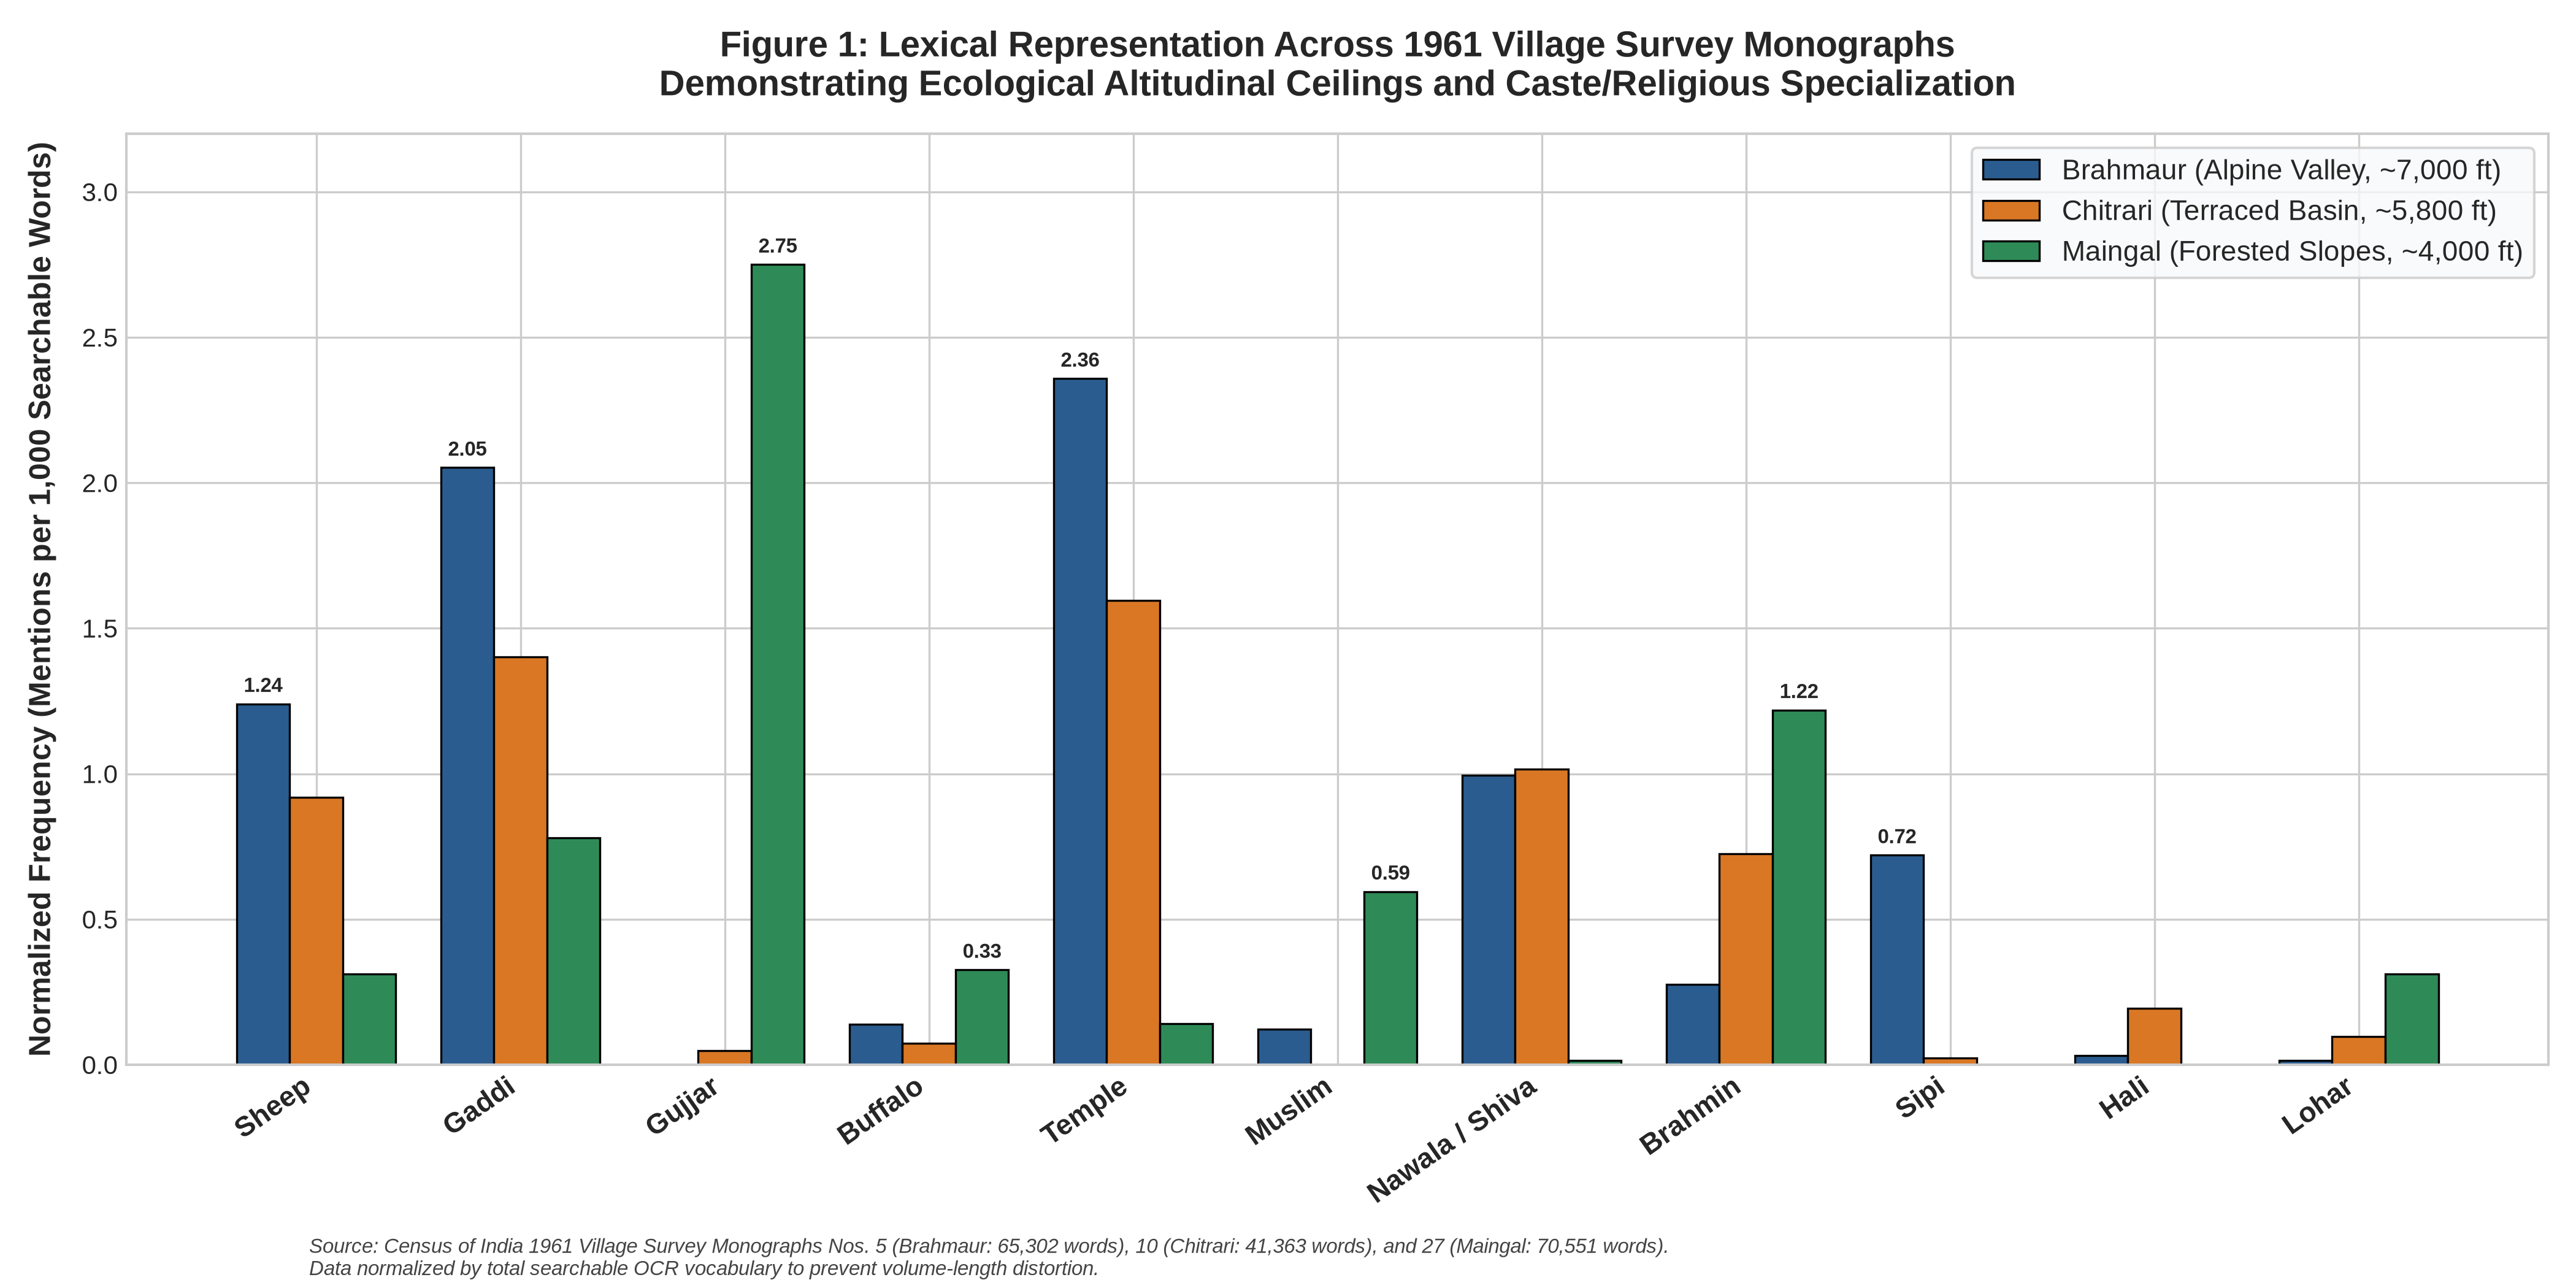
\includegraphics[width=0.95\textwidth]{outputs/figures/fig1_1961_village_mentions_normalized.png}
\caption{Normalized Relative Word Frequencies Across 1961 Village Survey Monographs (Mentions per 1,000 Searchable Words). Notice the sharp divergence: pastoral sheep and temples in alpine Brahmaur; land, temples, and Brahmins in terraced Chitrari; Gujjars, buffaloes, and Lohars in forested Maingal.}
\label{fig:norm_freq}
\end{figure}

\subsection{Finding 1: The Ecological Altitude Ceiling of Pastoral Production}
\begin{itemize}[leftmargin=*]
    \item \textbf{Observation:} Relative word frequencies indicate sheep prominence in Brahmaur (1.24/1k) and Gujjar dominance in Maingal (2.75/1k). Buffaloes appear 9 times in the Brahmaur survey text but count for 0 animals in the village livestock census, whereas Maingal holds 217 buffaloes.
    \item \textbf{Source Verification:} The Brahmaur survey text (p.~43) provides the explicit causal explanation:
    \begin{quote}
    \textit{``No one keeps a buffalo as the climate is not conducive to the proper rearing of buffalo. Once a villager brought a buffalo, but he was not happy with the experience as the milk yield suddenly dropped from 9 srs. to 4 srs. and the buffalo had to be taken to low hills before winter.''}
    \end{quote}
    \item \textbf{Comparison:} High-altitude Brahmaur ($\sim$7,000 ft) adapted to severe alpine cold through transhumant sheep and goats (4,484 head). Conversely, sub-Himalayan Maingal ($\sim$4,000 ft) supported intensive commercial buffalo dairying (Figure~\ref{fig:livestock}).
    \item \textbf{Interpretation:} Environmental altitude establishes a physiological boundary on pastoral capital. The susceptibility of water buffaloes to lactation collapse under alpine frost barred dairy transhumance into the upper Ravi, securing Gaddi monopoly over high-altitude sheep pastoralism while creating a lower-elevation ecological niche for Gujjars.
    \item \textbf{Alternative Explanation:} Cultural taboos against buffalo rearing among orthodox Hindus might be suggested; however, the source refutes this by recording that Gaddi villagers attempted buffalo rearing for commercial milk before economic failure forced abandonment.
    \item \textbf{Limitation:} The survey records lactation statistics for a single trial; historical longitudinal veterinary records across multiple households are unavailable.
\end{itemize}

\begin{figure}[H]
\centering
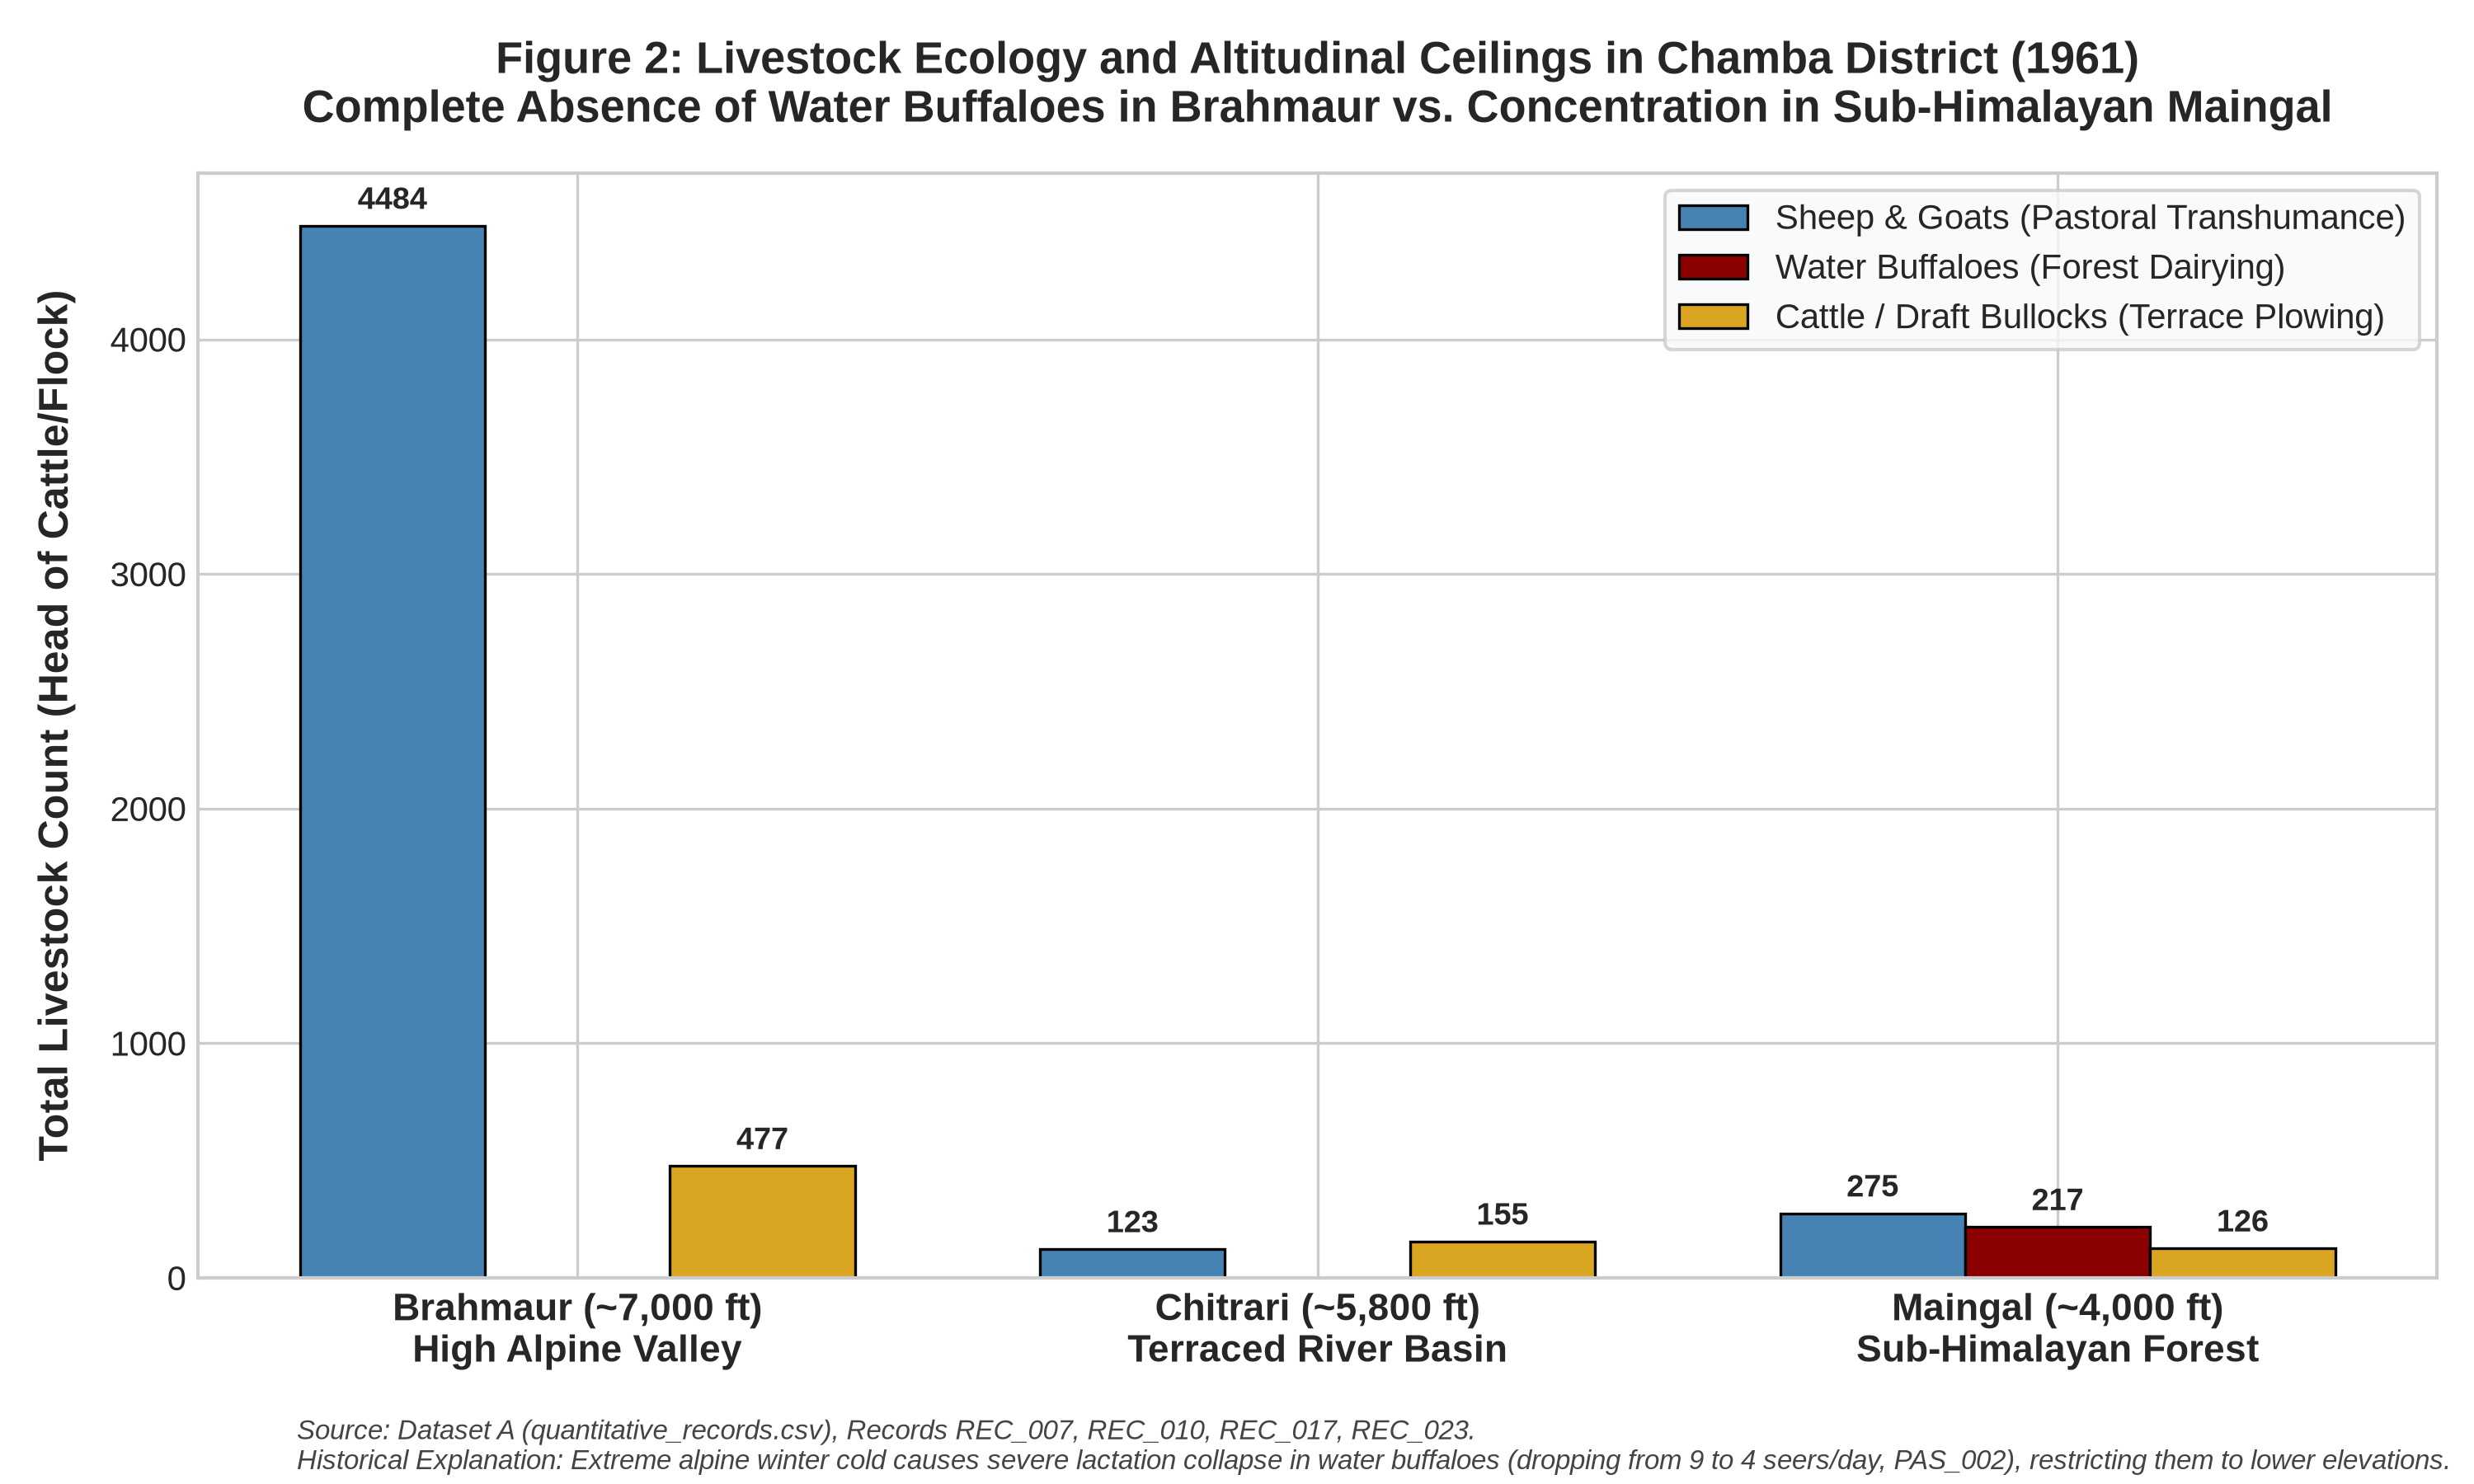
\includegraphics[width=0.85\textwidth]{outputs/figures/fig2_livestock_ecological_distribution.png}
\caption{Livestock Herd Composition Across the Micro-Ecological Zones (1961). Water buffaloes are completely barred from alpine Brahmaur ($\sim$7,000 ft) and concentrated in sub-Himalayan Maingal ($\sim$4,000 ft).}
\label{fig:livestock}
\end{figure}

\subsection{Finding 2: Village-Specific Caste Divisions of Labour and Artisan Reciprocity}
\begin{itemize}[leftmargin=*]
    \item \textbf{Observation:} Sipi mentions are concentrated in Brahmaur (0.72/1k; 47 mentions); Hali mentions in Chitrari (0.19/1k; 8 mentions); and Lohar blacksmith mentions in Maingal (0.31/1k; 22 mentions).
    \item \textbf{Source Verification:}
    \begin{enumerate}
        \item \textit{Sipis in Brahmaur (pp.~18, 24, 38, 44, 62):} Sipis (15 households / 119 persons) hold an indispensable tripartite monopoly:
        \begin{itemize}
            \item \textbf{Pastoral Wage Labour:} Serve as hired shepherds (\textit{pohals}) under formal contracts (free food, clothing, wool, a 2--4\% sheep dividend, and Rs.~2/month wages).
            \item \textbf{Textile Manufacture:} Shear sheep with hand shears (\textit{katar}), weave coarse tweed (\textit{pattu}) and blankets (\textit{gardu}), and tailor the traditional Gaddi frock (\textit{chola}) and rope sash (\textit{dora}).
            \item \textbf{Ritual Reciprocity:} Perform as ceremonial drummers (\textit{dholak}) during the Shiva \textit{Nawala}, receiving the sacrificial sheep's neck (\textit{ghardi}) and flour.
        \end{itemize}
        \item \textit{Halis in Chitrari (pp.~11--12):} Landed Brahmins (311 persons / 77\% of the village) hold vast terraced estates derived from historic temple grants dating to Raja Meru-Varman. Constrained by religious taboos against touching the plough, Brahmins relied on attached \textbf{Halis} (6 persons across 2 households) for field cultivation. Halis mobilized under the Arya Samaj, adopting the name \textit{Aryas--Halis} to contest untouchability.
        \item \textit{Lohars in Maingal (pp.~12, 33):} Two Lohar households (8 persons) maintain workshops fabricating and repairing iron ploughshares. In return, they receive non-monetary \textbf{khalian} fixed customary sheaves of unhusked grain delivered directly from the threshing floor (\textit{khala}) at each harvest.
    \end{enumerate}
    \item \textbf{Comparison:} Caste labour was strictly place-dependent. In pastoral Brahmaur, social relations centered on wool processing and sacrificial meat sharing. In agrarian Chitrari, relations were mediated by land tenure and plough taboos. In forested Maingal, relations operated through non-monetary jajmani tool maintenance.
    \item \textbf{Interpretation:} Mountain villages were not self-sufficient autarkies, but tightly integrated moral economies where upper-caste landholders were structurally dependent on specialized lower-caste technical and ritual labour.
    \item \textbf{Alternative Explanation:} One might assume that cash wages had replaced traditional services by 1961. The evidence disproves this: cash contracts (\textit{pohal} wages) co-existed directly with customary non-monetary grain (\textit{khalian}) and meat (\textit{ghardi}) barter.
    \item \textbf{Limitation:} The survey records institutional rules clearly, but omits day-to-day wage bargaining disputes between individual households.
\end{itemize}

\subsection{Finding 3: Inter-Religious Co-Existence and Trans-Pastoral Symbiosis}
\begin{itemize}[leftmargin=*]
    \item \textbf{Observation:} Maingal records high Muslim frequency (0.60/1k; 42 mentions), with 203 Muslim Gujjars (81.5\% of the sample population) co-existing with 34 Hindu Brahmins and 4 Rajputs. Chitrari records 0 Muslim residents, yet documents qualitative mentions of seasonal Gujjar camps.
    \item \textbf{Source Verification:}
    \begin{itemize}
        \item \textit{Maingal (pp.~12, 33):} Muslim Gujjars live in 13 dispersed forest hamlets in flat-roofed \textit{kothas}. They supply rich buffalo manure and draft animals to Brahmin cultivators, marketing commercial ghee in Chamba town, while maintaining peaceful social relations with Hindu farmers.
        \item \textit{Chitrari (p.~45):} Local cows yield negligible milk (4--8 chhataks/day). Villagers rely entirely on transhumant Muslim Gujjars camping on high alpine ridges (\textit{dhars}) during the monsoon to purchase fresh milk and butter.
    \end{itemize}
    \item \textbf{Comparison:} In Maingal, inter-religious co-existence took the form of \textbf{settled, shared village space}; in Chitrari, it took the form of \textbf{seasonal, high-altitude market exchange} between sedentary Hindus and mobile pastoral Muslims.
    \item \textbf{Interpretation:} Religious harmony in rural Chamba was sustained not by abstract tolerance, but by \textbf{material economic complementarity}. Muslim Gujjars and Hindu agriculturalists occupied non-competing ecological niches: Gujjars exploited forest and alpine pasture browsed by buffaloes, while Hindu Brahmins cultivated terraced cereals.
    \item \textbf{Alternative Explanation:} Communal tensions could have been suppressed by census investigators. However, the absence of land disputes is corroborated by spatial settlement patterns: Brahmin nucleated hamlets and Gujjar forest \textit{kothas} maintained independent water sources and grazing runs.
    \item \textbf{Limitation:} Oral histories of Gujjar conversion and migration dates were recorded without independent archival verification from princely Chamba court records.
\end{itemize}

\subsection{Finding 4: Bipartite Network of Economic Interdependence}

\begin{figure}[H]
\centering
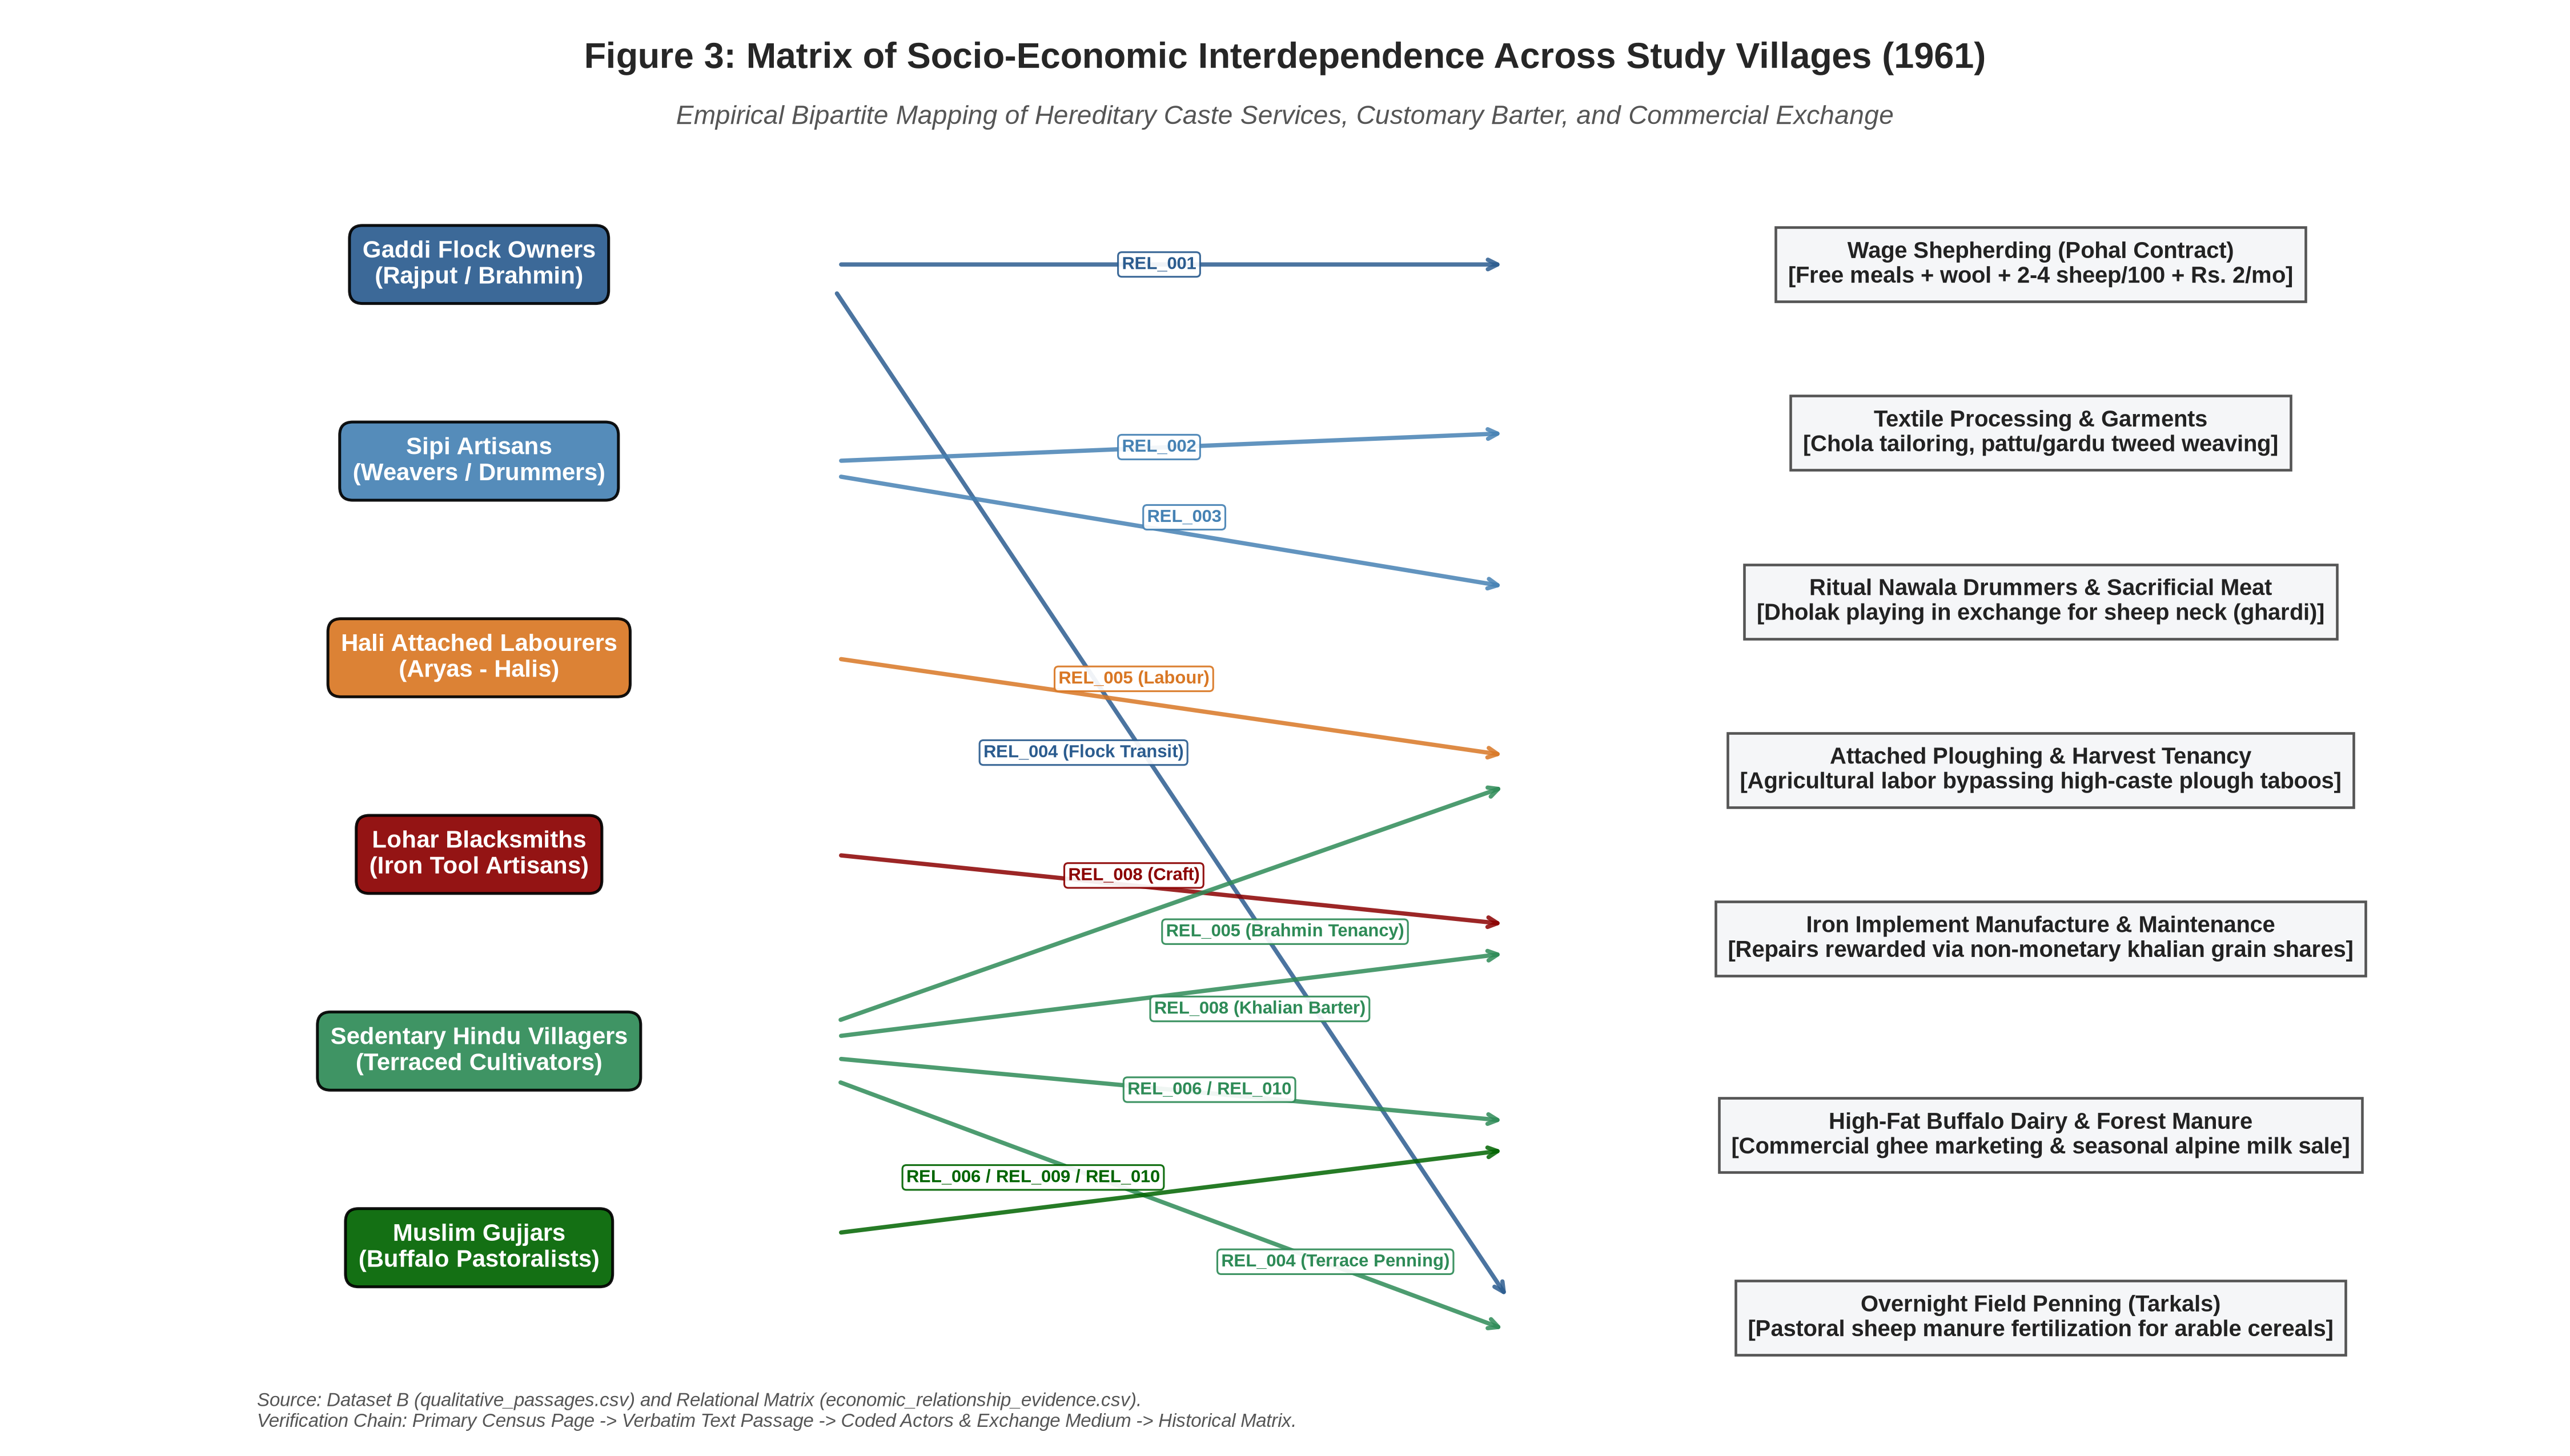
\includegraphics[width=0.95\textwidth]{outputs/figures/fig3_bipartite_economic_exchange.png}
\caption{Bipartite Interaction Matrix Mapping Verified Socio-Economic Interdependence Across Study Villages (1961). Each link represents explicit textual proof connecting caste/religious actors with specific exchange media.}
\label{fig:bipartite}
\end{figure}
The 12 verified exchange relationships substantiate that rural Chamba operated as a multi-tiered economy where monetary transactions, customary jajmani perquisites, and state-regulated ecological transfers functioned concurrently (Table~\ref{tab:relationships}).

\begin{table}[H]
\centering
\footnotesize
\caption{Verified Register of Documented Socio-Economic Exchange Relationships (1961)}
\label{tab:relationships}
\begin{tabularx}{\textwidth}{llp{3cm}p{3.5cm}X}
\toprule
\textbf{Rel.} & \textbf{Village} & \textbf{Actor 1 $\leftrightarrow$ Actor 2} & \textbf{Exchange Medium} & \textbf{Historical Significance} \\
\midrule
R-1 & Brahmaur & Gaddi Flock Owner $\leftrightarrow$ Hired Shepherd & Meals, wool, 2--4 sheep/100, Rs. 2/mo wages & Stratified contractual wage relations within pastoralism (Brahmaur Survey, p.~44). \\
R-2 & Brahmaur & Flock Owner $\leftrightarrow$ Sipi Weaver/Tailor & Sheared raw wool shares, food perquisites & Interdependence linking upper-caste sheep owners to lower-caste textile specialists (Brahmaur Survey, p.~38). \\
R-3 & Brahmaur & Brahmin Priest/Host $\leftrightarrow$ Sipi Musician & Sacrificed sheep neck (\textit{ghardi}), grain & Ritual reciprocity crossing caste boundaries during Shaivite \textit{Nawala} feasts (Brahmaur Survey, p.~62). \\
R-4 & Brahmaur & Gaddi Shepherds $\leftrightarrow$ Terraced Cultivators & Overnight sheep penning (\textit{tarkals}) for grain & Ecological nutrient transfer cycle via manure penning on fallow fields. \\
R-5 & Chitrari & Brahmin Landowner $\leftrightarrow$ Hali Ploughman & Tied crop-share tenancy and land access & Attached ploughing labour bypassing Brahmin taboos; Arya Samaj status contestation (Chitrari Survey, p.~11). \\
R-6 & Chitrari & Hindu Villagers $\leftrightarrow$ Nomadic Gujjars & Cash/grain purchase of milk on high \textit{dhars} & Seasonal inter-community trade supplying essential high-fat dairy nutrition (Chitrari Survey, p.~45). \\
R-7 & Chitrari & Shakti Devi Temple $\leftrightarrow$ Bensi Pipers & Customary grain perquisites \& temple stipend & Institutionalized temple service caste within sacred economy (Chitrari Survey, p.~32). \\
R-8 & Maingal & Cultivators $\leftrightarrow$ Lohar Blacksmiths & Customary unhusked grain (\textit{khalian}) & Customary non-monetary jajmani tool maintenance from threshing floor (Maingal Survey, p.~33). \\
R-9 & Maingal & Muslim Gujjars $\leftrightarrow$ Urban Bazaar Traders & Cash sale of clarified butter (\textit{ghee}) & Market integration transforming subsistence dairy into commercial commodity (Maingal Survey, p.~14). \\
R-10 & Maingal & Muslim Gujjars $\leftrightarrow$ Hindu Brahmins & Dung manure, bullock exchange, water rights & Inter-religious co-existence anchored in complementary production niches (Maingal Survey, pp.~12,~33). \\
R-11 & Regional & Gaddi Pastoralists $\leftrightarrow$ Dual Sovereign States & Summer grazing dues (Chamba) vs winter land tax & Trans-Dhaula Dhar mobility negotiating political borders and dual property rights (Ibbetson 1881, para.~498). \\
R-12 & Regional & Families $\leftrightarrow$ Rehara Silversmiths & Cash fee per tola silver crafted + metal scrap & Craft specialization converting pastoral livestock profits into portable dowry savings (Brahmaur Survey, p.~24). \\
\bottomrule
\end{tabularx}
\end{table}

---

\section{Material Culture and Vernacular Oral Evidence}

\subsection{Material Culture as Technological Anchors}
Material artifacts physically embodied the social division of labour and ecological adaptations:
\begin{enumerate}[leftmargin=*]
    \item \textbf{The Wooden Plough (\textit{Hal}) and Iron Share:} Lightweight wooden frame suited for steep terraced slopes, socketed with an iron share forged by Lohars. It physically embodied the plough taboo separating Brahmin landowners from attached Hali labourers.
    \item \textbf{The Conical Basket (\textit{Kilta}):} Back-borne transport technology woven from bamboo, enabling women to carry heavy manure loads to terraced fields.
    \item \textbf{Iron Shearing Scissors (\textit{Katar}):} Hand-forged shears operated exclusively by Sipis to clip wool from Gaddi sheep flocks thrice annually.
    \item \textbf{The Wool Pit Loom (\textit{Rachh}):} Frame looms operated by Sipi weavers to produce coarse tweed (\textit{pattu}) and blankets (\textit{gardu}), tailored into the Gaddi \textit{chola} and \textit{dora}.
    \item \textbf{Traditional Silver Ornaments (\textit{Chiri}, \textit{Ralu}, \textit{Kanbali}):} Heavy silver jewelry crafted by Reharas, converting volatile pastoral livestock profits into portable savings and dowry (\textit{stridhana}).
    \item \textbf{The Gujjar \textit{Kotha} and Field \textit{Machan}:} Low flat-roofed stone-timber dwellings housing both humans and buffalo herds, paired with elevated stilt platforms (\textit{machans}) used to guard maize crops against mountain wildlife.
\end{enumerate}

\subsection{Vernacular Oral History as the Emotional Archive}
Devanagari folk verses mined from the village survey monographs provide indigenous perspectives counterbalancing administrative prose:
\begin{enumerate}[leftmargin=*]
    \item \textbf{The Transhumant Husband's Absence (Chitrari, pp. 72--73):} Sung by Gaddi women left behind during summer transhumance; reveals the physical torment of barefoot ascent up thorny pastures (\textit{``nange pairin main dhar chadhi jaandi''}) and structural dependence on the village revenue accountant (\textit{Patwari}) to write letters.
    \item \textbf{The Sacrificial Vow (\textit{Shiv Ainchali}, Brahmaur, p. 66):} Documents the sacrificial offering of 84 sheep and goats to Lord Shiva; details the multi-caste assembly where Brahmin priests, trance mediums (\textit{chelas}), and Sipi drummers share sanctified meat.
    \item \textbf{The Shepherd's Death on the Frozen Pass (\textit{Bhohku Git}, Brahmaur, p. 58):} Documents the death of shepherd Bhukhu in an unseasonal blizzard on the high mountain pass (\textit{jot}), mourning his lost flock and relaying news through trans-Himalayan Lahauli caravaneers.
\end{enumerate}

---

\section{Source Criticism, Methodological Biases, and Limitations}

A critical historical methodology demands explicit acknowledgment of source limitations:
\begin{enumerate}[leftmargin=*]
    \item \textbf{The ``Absence Fallacy'' in OCR Corpora:} Lexical search tools cannot distinguish between the absence of a word in a text layer and the historical absence of a community in a territory. The zero occurrences of \textit{Gujjar} in Brahmaur village text must be qualified by regional transhumance patterns.
    \item \textbf{Colonial Census Seasonality:} The 1881 and 1931 censuses were conducted in February---the middle of winter. This seasonal timing caught transhumant Gaddis and Gujjars in low-elevation winter camps in Kangra and Jammu, artificially deflating high-altitude Himalayan district counts.
    \item \textbf{Scale Mismatch:} Macro-provincial tables cannot be disaggregated into individual villages; conversely, micro-village monographs cannot be uncritically generalized to the entire Western Himalayas without comparative control.
    \item \textbf{Categorical Drift Across Eras:} While craft categories like \textit{Lohar} remain directly comparable across 1881, 1931, and 1961, pastoralism and tenancy are only partly comparable due to shifts from hereditary caste definitions to economic dependency categories.
\end{enumerate}

---

\end{document}
